\documentclass[notes]{subfiles}

\begin{document}
	\addcontentsline{toc}{section}{1.8 - Continuity}
	\refstepcounter{section}
	\setcounter{section}{8}
	\fancyhead[RO,LE]{\bfseries \large\nameref{cs18}} 
	\fancyhead[LO,RE]{\bfseries \currentname}
	\fancyfoot[C]{{}}
	\fancyfoot[RO,LE]{\large \thepage}	%Footer on Right \thepage is pagenumber
	\fancyfoot[LO,RE]{\large Chapter 1.8}

\section*{Continuity}\label{cs18}
	\subsection*{Before Class}
	\addcontentsline{toc}{subsection}{Before Class}
	\subsubsection*{The Definition}
	\addcontentsline{toc}{subsubsection}{The Definition}
		\begin{defn}[Continuity]
			A function is \textbf{continuous at input} $a$ if 
			\showto{ins}{
				\[\lim_{x\to a} f(x) = f(a)\] \\
			}
			\showto{st}{
				\\ \\ \\ \\
			}
			 If this condition fails, then $f$ is said to be 
			\showto{ins}{
				\fbox{discontinuous at input} $a$.
			}
			\showto{st}{
				\blank{2.5}.\\ \\
			}
			$f$ is \textbf{continuous on an interval} if it is
			\showto{ins}{
				\fbox{continuous at every number in the interval}.
			}
			\showto{st}{
				\blank{3.5}.
			}
		\end{defn}
			\vs{.25}
			
		\begin{rmk}[Conditions for Continuity]
			Continuity of a function requires three things:
			\showto{ins}{
				\begin{enumerate}
					\item \fbox{$a$ is in the domain of $f$}
					\item \fbox{$\ds\lim_{x\to a} f(x)$ exists}
					\item \fbox{$\ds\lim_{x\to a} f(x) = f(a)$}
				\end{enumerate}
			}
			\showto{st}{ \\ \\
				\begin{enumerate}
				\setlength\itemsep{15pt}
					\item \blank{4} 
					\item \blank{4}
					\item \blank{4}
				\end{enumerate}
			}
		\end{rmk}
			\vs{.25}
		\begin{question}
			Look back at \S1.5 and the conditions for the existence of a limit.  What connections can you draw between the existence of a limit and the conditions for continuity?
		\end{question}	
			\vs{1}
			\newpage
			
		\begin{ex}
		Use the graph to find the following:
		\begin{center}
			\begin{tikzpicture}
				\begin{axis}[
					scale = 1.5,
					every tick label/.append style={font=\small},
					axis x line = middle,
					axis y line = middle,
		    			every axis y label/.style={at={(ticklabel cs:1.15)}},
		    			ytick = {-4, -2, -3, -1, 1, 2, 3, 4},
					y label style={at={(axis description cs:.5,1.15)},anchor=north},
		    			ylabel = {$f(x)$},
		    			ymin = -5, ymax = 5,
	    				every axis x label/.style= {at ={(ticklabel cs:1)}},
	    				xtick = {-4,-3,-2,-1,1,2,3,4},
	    				x label style={at={(axis description cs:1.1,.5)},anchor=east},
	    				xlabel = {$x$},
	    				xmin = -5, xmax = 5			
					]
					\addplot[<-,thick,smooth,domain = 1.4:3.] {4/(x-1)-5};
					\addplot[->,thick,smooth,domain = 3.:4.9] {x-6};
					\addplot[<-,thick,smooth, domain = -4.9:1]  {2^x -4};
					\coordinate (circle1) at (1,-2);
					\coordinate (circle2) at (3,-3);
					\coordinate (circle3) at (3,2);
				\end{axis}
					\fill[white] (circle1) circle (.1);
					\draw[thick] (circle1) circle (.1);
					\fill[white] (circle2) circle (.1);
					\draw[thick] (circle2) circle (.1);
					\fill (circle3) circle (.1);
			\end{tikzpicture}
		\end{center}\vspace*{20pt}
		\begin{minipage}{\textwidth}
			\begin{multicols*}{3}
			\begin{enumerate}[(a)]
				\item $\ds \lim_{x\to 1^+} f(x)$\\[50pt]
				\item $\ds \lim_{x\to 1^-} f(x)$\\[50pt] 
				\item $\ds \lim_{x\to 1} f(x)$\\[50pt] 
				\item Is $f$ continuous at $x =1 $?\\[50pt]
					\columnbreak
				\item $\ds \lim_{x\to 3^+} f(x)$\\[50pt] 
				\item $\ds \lim_{x\to 3^-} f(x)$\\[50pt]  
				\item $\ds \lim_{x\to 3} f(x)$\\[50pt] 
				\item Is $f$ continuous at $x =3 $?\\[50pt]
					\columnbreak
				\item $\ds \lim_{x\to 0^+} f(x)$\\[50pt] 
				\item $\ds \lim_{x\to 0^-} f(x)$\\[50pt]  
				\item $\ds \lim_{x\to 0} f(x)$\\[50pt] 
				\item Is $f$ continuous at $x =0 $?\\[50pt]
			\end{enumerate}
				\raggedcolumns
			\end{multicols*}
		\end{minipage}
		\end{ex}
			\newpage

		\begin{rmk}[Types of Discontinuities]
			There are three kinds of discontinuities which we will encounter:
			\showto{ins}{
				\begin{itemize}
					\item \fbox{Vertical Asymptote}
					\item \fbox{Jump Discontinuity}
					\item \fbox{Removable Discontinuity}
				\end{itemize}			
			}
			\showto{st}{ \\ \\
				\begin{itemize}
				\setlength\itemsep{15pt}
					\item \blank{3}
					\item \blank{3}
					\item \blank{3}
				\end{itemize}
			}
		\end{rmk}
			
		\begin{ex}
			Sketch an example of each of the three kinds of discontinuities.
		\end{ex}
			\vs{1}

		\begin{defn}[Continuity from the Right and Left]
			A function $f$ is said to be \textbf{continuous from the right} at input $a$ if
			\showto{ins}{
				\[\lim_{x\to a^+} f(x) = f(a)\]
			}
			\showto{st}{
				\\ \\ \\ \\
			}
			and $f$ is \textbf{continuous from the left} at input $a$ if 
			\showto{ins}{
				\[\lim_{x\to a^-} f(x) = f(a)\]
			}
			\showto{st}{
				\\ \\
			}
		\end{defn}	
		
			\newpage
		
		\subsubsection*{Pre-Class Activities}
		\addcontentsline{toc}{subsubsection}{Pre-Class Activities}	
		\begin{ex}
			Use the graph below to answer the following questions:\\
			\begin{minipage}{3in}
				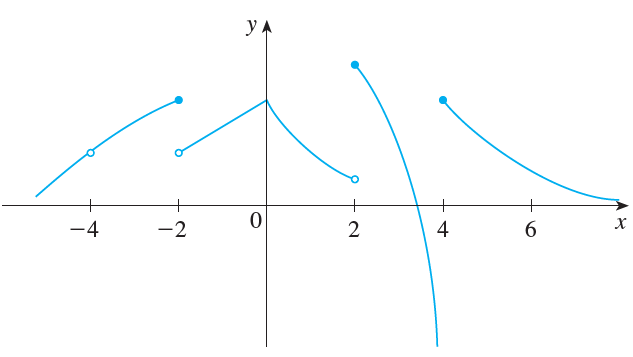
\includegraphics[scale = .58]{1.8fig1}
			\end{minipage}
			\begin{minipage}{3.8in}
				\begin{enumerate}[(a)]
					\item State the numbers at which $f$ is discontinuous, and classify each as a \emph{vertical asymptote}, \emph{jump discontinuity}, or \emph{removable discontinuity}.
					\item For each of the numbers in (a), determine whether $f$ is right-continuous, left-continuous, or neither.  
					\item Use interval notation to write where $f$ is continuous.
				\end{enumerate}
			\end{minipage}
		\end{ex}
			\vs{1}
			
		\begin{ex}
			Sketch the graph of a function $f$ that is continuous everywhere, but is:
				\begin{itemize}
					\item Discontinuous at $x = 5$
					\item Left-continuous at $x = -1$
					\item Has a removable discontinuity at $x = 3$.
				\end{itemize}
		\end{ex}
			\vs{1}

		\newsec
	\subsection*{In-Class}
	\addcontentsline{toc}{subsection}{In-Class}

		\begin{ex}
			Show that $\llbracket x \rrbracket$ is right-continuous, but not left-continuous at integer values.
		\end{ex}
			\vs{2}
			\newpage
			
		\begin{ex}
			Show that the function $f(x) = 3+\sqrt{1-x^2}$ is continuous on the interval $[-1,1]$.
		\end{ex}
			\vs{2}
			
	\subsubsection*{Useful Results}
	\addcontentsline{toc}{subsubsection}{Useful Results}
		\begin{thm}[Properties of Continuous Functions]
			If $f$ and $g$ are continuous at $a$, and if $c$ is a constant, then the following functions are all continuous at $a$:
			\showto{ins}{
				\begin{enumerate}
					\item $f \pm g$
					\item $cf$
					\item $fg$
					\item $\dfrac{f}{g}$, for $g\neq 0$
					\item $f\circ g$
				\end{enumerate}
			}
			\showto{st}{\\ \\
				\begin{enumerate}
				\setlength\itemsep{15pt}
					\item \blank{3}
					\item \blank{3}
					\item \blank{3}
					\item \blank{3}
					\item \blank{3}
				\end{enumerate}
			}
		\end{thm}
			\vs{.25}
			\newpage
			
		\begin{ex}
			Prove the first property of continuous functions.
		\end{ex}
			\vs{2}
			
		\begin{question}
			Can you prove the remaining 4 properties?
		\end{question}
			\vs{.5}
			
		\begin{thm}[Types of Continuous Functions]
			The following functions are continuous on their domain:
			\showto{ins}{
				\begin{itemize}
					\item Polynomials
					\item Rational Functions
					\item Root functions
					\item Trigonometric Functions
				\end{itemize}		
			}
			\showto{st}{ \\ \\
				\begin{itemize}
				\setlength\itemsep{15pt}
					\item \blank{3}
					\item \blank{3}
					\item \blank{3}
					\item \blank{3}
				\end{itemize}
			}
		\end{thm}
			\newpage
			
		\begin{ex}
			Find the interval(s) on which the following functions are continuous
			\begin{enumerate}[(a)]
				\item $f(x) = x^{67}-47.521x^{51}+719$
					\vs{1}
					
				\item $g(x) = \dfrac{x^2+2x+17}{x^2-1}$
					\vs{1}
					
				\item $h(x) = \sqrt{x} + \dfrac{x+1}{x-1} + \dfrac{x+1}{x^2+1}$
					\vs{1}
					
				\item $\cos\lrpar{\dfrac{1}{x}}$
					\vs{1}
					
			\end{enumerate}
		\end{ex}
			\newpage
			
	\subsubsection*{The Intermediate Value Theorem}
	\addcontentsline{toc}{subsubsection}{The Intermediate Value Theorem}
		\begin{thm}[Intermediate Value Theorem]
			Suppose that $f$ is continuous on the closed interval $[a,b]$, and let $N$ be any number between $f(a)$ and $f(b)$, where $f(a)\neq f(b)$.  Then,
			\showto{ins}{
				\fbox{there exists a number $c$ in $(a,b)$ such that $f(c) = N$.}
			}
			\showto{st}{
				\\ \\ \\
			}
		\end{thm}
		Here is a sketch illustrating why the Intermediate Value Theorem is true:
			\vs{1}	

		\begin{question}
			Why does a function need to be continuous in order to guarantee the conclusion of the Intermediate Value Theorem?  Sketch a graph to support your idea.
		\end{question}
			\vs{1}
			\newpage
			
		\begin{ex}
			Show that the equation $4x^3-6x^2+3x-2 = 0$ has a root between 1 and 2.
		\end{ex}
			\vs{1}
			
		\begin{ex}
			For what value of the constant $c$ is the function $f$ continuous on $(-\infty,\infty)$?
			\[f(x) = \begin{cases} cx^2+2x & x < 2 \\ x^3-cx & x\geq 2\end{cases}\]
		\end{ex}
			\vs{1}
			\newpage
			
	\subsection*{After Class}
	\addcontentsline{toc}{subsection}{After Class}
		\begin{ex}
			Use the graph below to answer the following questions:\\
			\begin{minipage}{3in}
				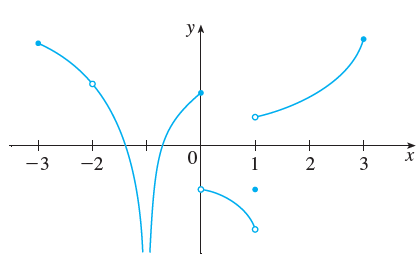
\includegraphics[scale = .85]{1.8fig2}
			\end{minipage}
			\begin{minipage}{3.8in}
				\begin{enumerate}[(a)]
					\item State the numbers at which $f$ is discontinuous, and classify each as a \emph{vertical asymptote}, \emph{jump discontinuity}, or \emph{removable discontinuity}.
					\item For each of the numbers in (a), determine whether $f$ is right-continuous, left-continuous, or neither.  
					\item Use interval notation to write where $f$ is continuous.
				\end{enumerate}
			\end{minipage}
		\end{ex}
			\vs{1}
		\begin{ex}
			Find the numbers at which $g$ is discontinuous.  At which of these numbers is $f$ right-continuous, left-continuous, or neither?
				\[ g(x) = \begin{cases}x^2 + 1 & x \leq 1\\ 3-x & 1 < x \leq 4 \\ \sqrt{x} & x > 4 \end{cases}\]
		\end{ex}
			\vs{1}
			\newpage
			
		\begin{ex}
			Find values of $a$ and $b$ that make $f$ continuous everywhere.
				\[f(x) = \begin{cases}\dfrac{x^2-4}{x-2} & x < 2 \\ ax^2 - bx + 3 & 2\leq x < 3 \\ 2x - a + b & x \geq 3 \end{cases}\]
		\end{ex}
			\vs{1}
		
		\begin{ex}
			Suppose $f$ and $g$ are continuous function such that $g(2) = 6$ and $\ds \lim_{x\to 2} [3f(x) + f(x)g(x)] = 36$.  What is $f(2)$?
		\end{ex}
			\vs{1}
			\newpage
			
		\begin{ex}
			Show that the equation $\sqrt{x-5} = \dfrac{1}{x+3}$ has at least one real root.
		\end{ex}
			\vs{1}
	\clearpage
\end{document}